\documentclass{article}

\author{Teddy Krulewich}
\title{\vspace{-4em}HW1 ME5501 – Robotics and Unmanned Systems}

\usepackage{graphicx}
\graphicspath{ {images/} }


\usepackage[utf8]{inputenc}
\usepackage{minted}
\usepackage{hyperref}
\usepackage{xcolor}
\definecolor{bg}{rgb}{0.95,0.95,0.95}
\usepackage{caption}
\usepackage{mdframed}

\begin{document}
\maketitle

\section*{Problem 1}

Using the map shown below, generate the visibility graph (include the start and end nodes). 
Additionally, show the reduced visibility graph with a different color (i.e. blue for reduced graph, 
black for remaining standard edges). You do not need to compute the edge costs. 

\begin{figure}[h]
    \centering
    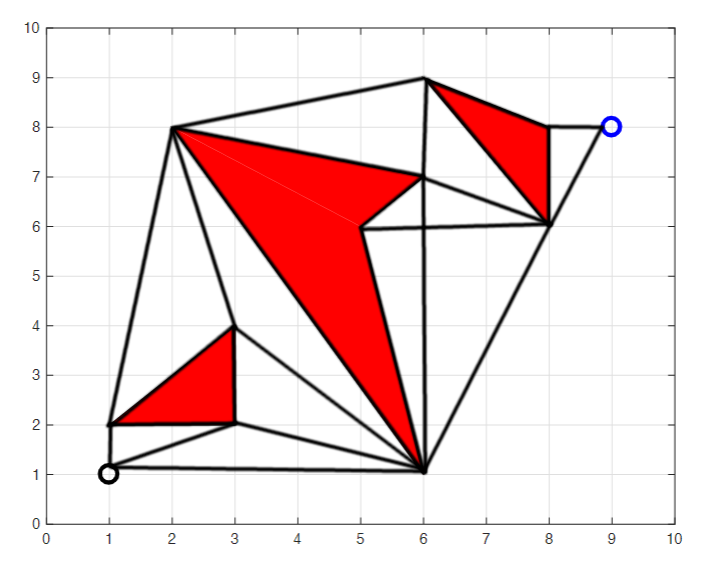
\includegraphics[width=6cm]{question1-visibility.png}
    \caption*{Visibility Graph}
\end{figure}

\begin{figure}[h]
    \centering
    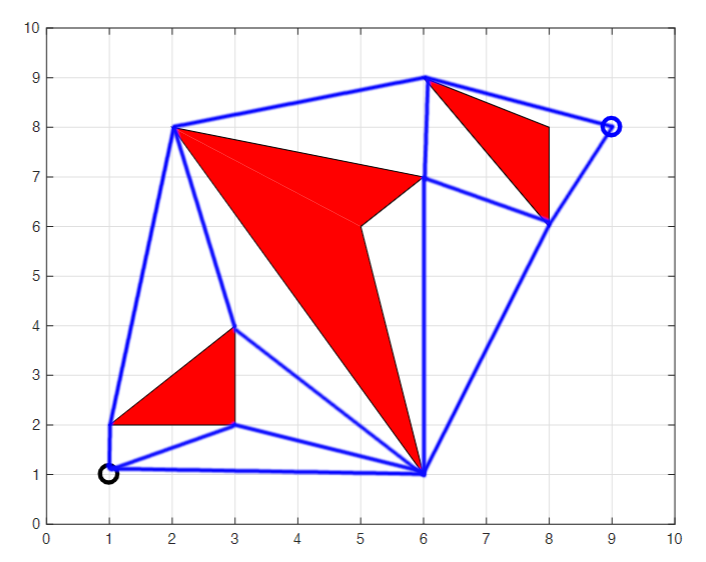
\includegraphics[width=6cm]{question1-reduced-visibility.png}
    \caption*{Reduced Visibility Graph}
\end{figure}

\section*{Problem 2}

Using the Python Class tutorial available at \url{https://docs.python.org/3/tutorial/classes.html},
create a class called node that has the following instance variables, x, y, parent\_cost, and index
Provide your short Python script that contains this class. 

\begin{mdframed}[backgroundcolor=bg]
\begin{minted}{python}
class Node:
    def __init__(self, x: float, y: float, 
        parent_node, index : int):
        
        self.x = x
        self.y = y

        self.parent_node = parent_node
        self.index = index

        self.cost = math.inf
    
    def distance(self, other) -> float:
        return math.sqrt(
            (self.x - other.x)**2 + (self.y - other.y) ** 2 )
    
    def __lt__(self, other) -> bool:
        return self.cost < other.cost
\end{minted}
\end{mdframed}

\section*{Problem 3}
 
Using the map shown below, show the reduced visibility graph along with the Euclidean distance for 
each edge. Highlight the shortest path from the start (1,1) to the goal (9,8). 

\begin{figure}[h]
    \centering
    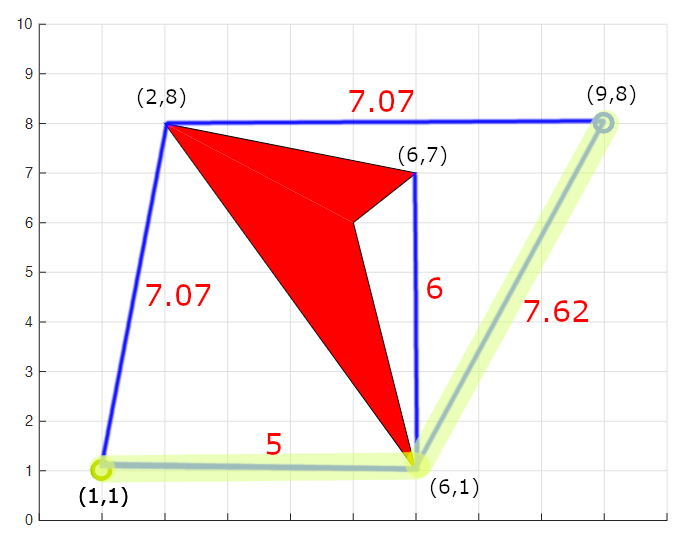
\includegraphics[width=5cm]{question3.png}
    \caption*{Reduced Visibility Graph\\Shortest path is highligted in yellow!}
\end{figure}

\newpage
\section*{Problem 4}

Given the following map parameters, generate a figure similar to the one shown in which you are 
computing each node index and plotting the index at the corresponding node location. The node 
index is simply the unique name/value associated with the node. You need to write your Python 
script such that any node location (x and y pair) returns the node index. I.e. simply making counter 
that plots at each node location will not work. Use the equation(s) developed in class to assist in this 
problem. This node index is crucial in generating grid-based path planning techniques. A small 
function that computes the node index is an efficient method for computing the index. 

\bigskip
\noindent Grid Spacing = 0.5 \\
Min X = 0  Max X = 10 (include both 0 and 10 in your grid) \\
Min Y = 0  Max Y = 10

\bigskip
\noindent Notes:

\bigskip
\noindent When generating the x and y values (that span from 0 to 10), the NumPy command arange is 
particularly useful. Make sure that you capture the end point by adding an extra “grid\_size” onto the 
end value. 

\bigskip
\begin{mdframed}[backgroundcolor=bg]
\begin{minted}{python}
Matplotlib.text(x, y, str(int(number to display)),
    color="red", fontsize=8)
\end{minted}
\end{mdframed}
\bigskip
\noindent is a good function to use to stick the text in the figure.

\bigskip
As discussed in class I did inplement a function to get an index from (x,y) coordinates,
however I opted to generate the indicies differently, when creating the grid

\bigskip
\noindent The following code gets an index from (x, y) coordinates
\begin{mdframed}[backgroundcolor=bg]
\begin{minted}{python}
def get_node_index(self, x: float, y : float) -> int:
    """Gets index of node at an x,y coordinate"""    
    index = (y - self.min_y) / self.spacing 
        (self.max_x / self.spacing + 1) +
        x / self.spacing
    
    return int(index)
\end{minted}
\end{mdframed}
In order to actually draw the grid, I assigned a all Nodes an index when the grid is created.
I then call the Grid.draw() method which looks like this:
\begin{mdframed}[backgroundcolor=bg]
\begin{minted}{python}
def draw(self):
    """draws the grid with node indicies displayed in their 
    corresponding (x, y) coordinates"""

    for node in self.Nodes:
        plt.text(node.x, node.y, str(node.index), 
            color="red", fontsize=8, 
            horizontalalignment="center", 
            verticalalignment = "center")  
    
    plt.xlim([self.min_x - self.spacing, 
        self.max_x + self.spacing])

    plt.ylim([self.min_y - self.spacing,
        self.max_y + self.spacing])
    
    plt.xticks(ticks = [ x for x in 
        np.arange(self.min_x, 
        self.max_x + self.spacing,
        self.width / 5.0)])
        
    plt.yticks(ticks = [ y for y in 
        np.arange(self.min_y,
        self.max_y + self.spacing,
        self.height / 5.0)])

    plt.show()
\end{minted}
\end{mdframed}

\newpage
\noindent The entire code may be found in week1.py. An image of the execution is seen below.


\begin{figure}[h]
    \centering
    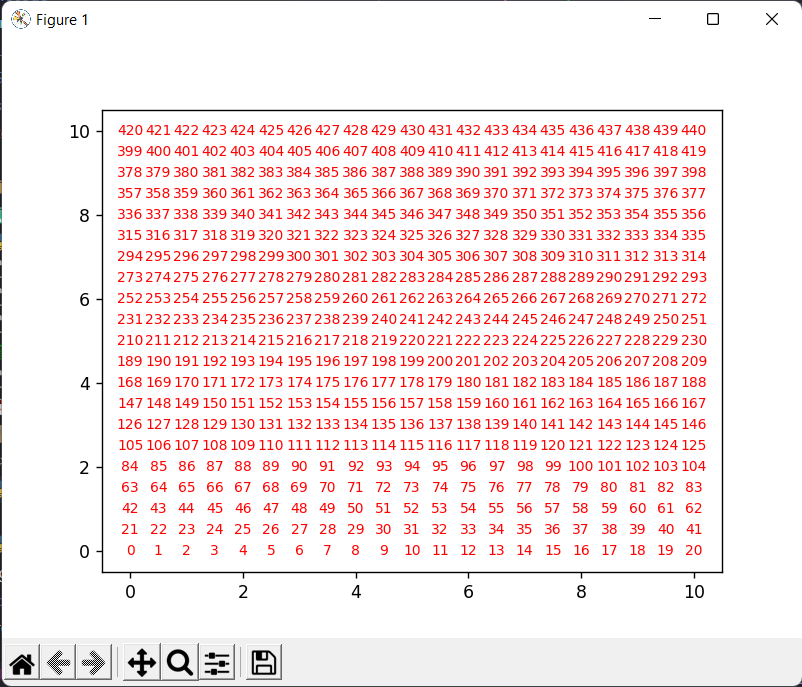
\includegraphics[width=\textwidth]{question4.png}
\end{figure}

\section*{Problem 5}
 
Create a function that calculates the distance from one node to another. Pass two nodes to the 
function and return the Euclidean distance. Test your function by having it calculate the distance 
from (2,1) to (3,2). Make sure the answer is correct. 
\bigskip
\noindent Submit your Python code.
\begin{mdframed}[backgroundcolor=bg]
\begin{minted}{python}
# the method below is defined within the node class
def distance(self, other):
    """Returns the euclidean distance between two nodes"""
    return math.sqrt(
        (self.x - other.x)**2 + (self.y - other.y) ** 2 )


node1 = Node(2, 1, None, 0)
node2 = Node(3, 2, None, 0)

print(node1.distance(node2))
\end{minted}
\end{mdframed}

\noindent\rule{\textwidth}{0.4pt}\\
\textbf{Output: 1.4142135623730951}


\end{document}